% vim: spelllang=es

\chapter{Investigación previa}

La propuesta para el sistema de plugins asumía que se iba a implementar con un
método que cubriré posteriormente denominado \emph{cargado dinámico}. Esto se
debe a razones de rendimiento, pero el método también incluye otros problemas
importantes, principalmente relacionados con seguridad. Por ello, es una buena
idea considerar las alternativas existentes para el PDK, en caso de que hubiera
alguno con la misma eficiencia pero menos vulnerabilidades.

Los requerimientos mínimos a tener en cuenta son los siguientes:

\begin{itemize}
    \item Debe ser posible añadir y quitar plugins tanto en el inicio del
        programa como durante su ejecución.

    \item Disponibilidad y madurez en el ecosistema de Rust.

    \item Soporte multi-plataforma: Windows, MacOS y Linux.

    \item No debe tener un impacto excesivo en el rendimiento. Esto significa
        que los eventos no se pueden copiar en ningún momento.

\end{itemize}

Y opcionalmente:

\begin{itemize}
    \item Maximizar la seguridad en lo posible, como se especifica en la sección
        \ref{sec:security}.

    \item Debería ser retro-compatible con el código ya existente, como indica la
        sección \ref{sec:compat}.

    \item Minimizar el esfuerzo necesario para reescribir los conectores para el
        nuevo sistema de plugins.

\end{itemize}

\section{Seguridad}\label{sec:security}

Muchas de las tecnologías que se pueden aplicar para un sistema de plugins usan
código \unsafe. Técnicamente, esto no es necesariamente un problema si la
implementación está autocontenida y auditada exhaustivamente, pero se pierden
algunas garantías que proporcionadas por Rust, incrementando el coste de
mantenimiento de la librería.

Asegurarse de que la implementación es segura implica una cantidad
considerablemente mayor de trabajo, aun cuando existen herramientas como
MIRI\footnote{\url{https://github.com/rust-lang/miri}} --- que integraría en
Tremor en caso de tener que recurrir a \unsafe.

\section{Retro-compatibilidad}\label{sec:compat}

\section{Tecnologías a considerar}

\subsection{Lenguajes de \scripting}

\subsection{Comunicación Inter-Proceso}

\begin{figure}
    \centering
    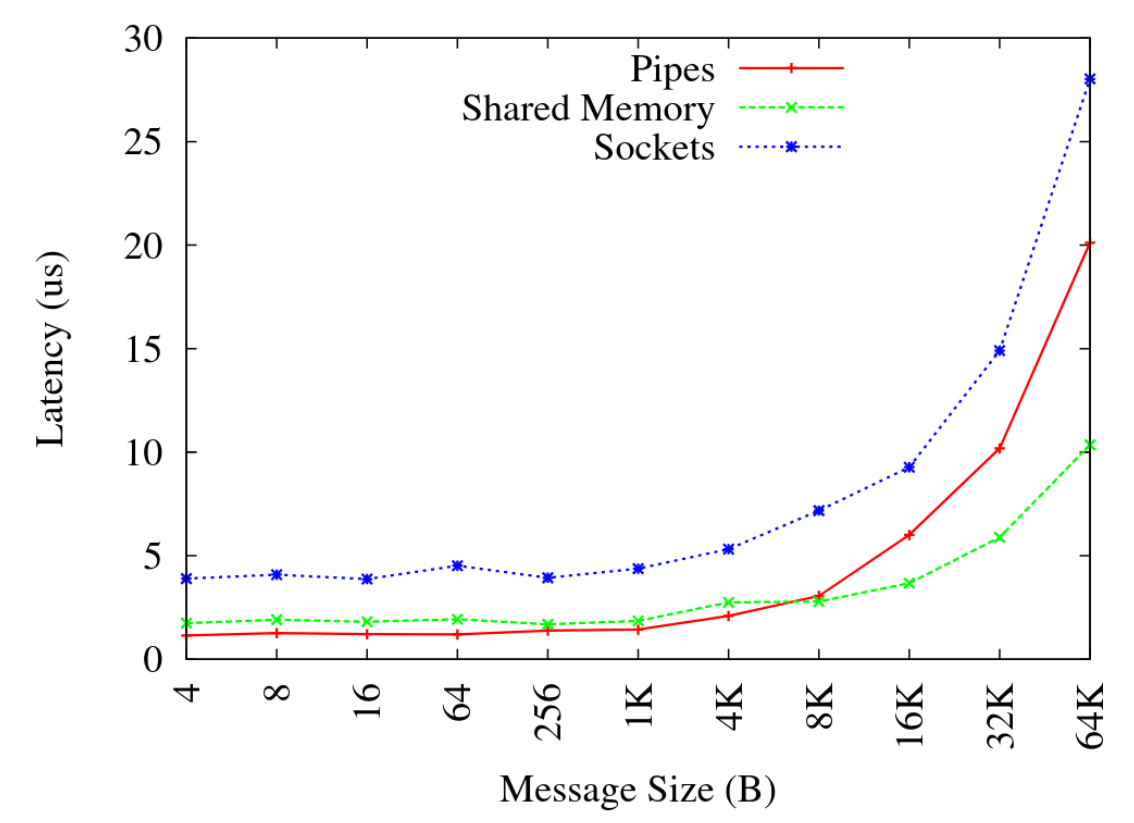
\includegraphics[width=10cm]{./Imagenes/venkataraman2015evaluation1.png}
    \caption{Latencia vs. Tamaño de Mensaje \cite{venkataraman2015evaluation}}%
    \label{fig:ipc_comparison1}
\end{figure}

\begin{figure}
    \centering
    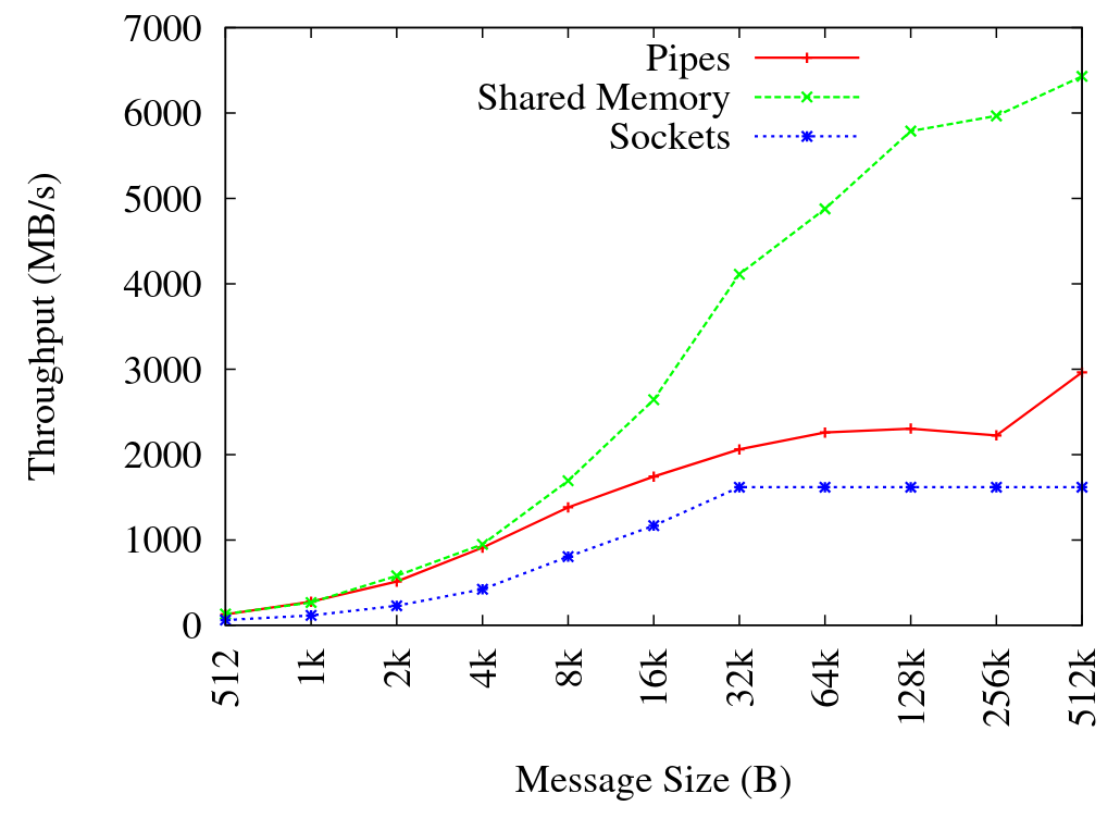
\includegraphics[width=10cm]{./Imagenes/venkataraman2015evaluation2.png}
    \caption{Rendimiento vs. Tamaño de Mensaje \cite{venkataraman2015evaluation}}%
    \label{fig:ipc_comparison2}
\end{figure}

\subsection{Cargado dinámico}

\subsection{WebAssembly}

\subsection{eBPF}

\section{Conclusión}

\begin{figure}
    \centering
    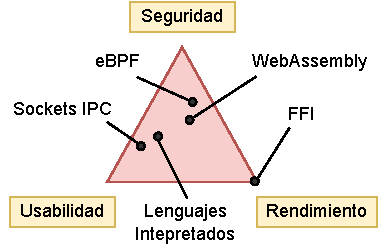
\includegraphics[width=10cm]{./Imagenes/triangle.pdf}
    \caption{Ejemplo de uso de Tremor}%
    \label{fig:tech_triangle}
\end{figure}
